% Sample file for KONA
% For ASCII pLaTeX2e
% This file requires article.cls
% 2017.01.13 by Nakanishi Printing Co., Ltd
% 2017.06.26 modified by Hao Shi, MSM, University of Twente, the Netherlands
% 2019.01.10 modified by Nakanishi Printing Co., Ltd

\documentclass[twocolumn, 10pt]{article}
\usepackage{amsmath,amssymb}
\usepackage{graphicx}
\usepackage[format=hang,labelfont=bf,textfont=small,singlelinecheck=false,justification=raggedright,margin={12pt,12pt},figurename=Fig.]{caption}
\usepackage{titlesec}
\usepackage{textcomp}


%%%%%%%%%%%%%%%%%%%%%%%%%%%%%%%%%%%%%%%%
\makeatletter
\def\affiliation#1{\gdef\@affiliation{#1}}
\def\abstract#1{\gdef\@abstract{#1}}
\def\graphabst#1{\gdef\@graphabst{#1}}
\def\keywords#1{\gdef\@keywords{#1}}
\def\corresp#1{\gdef\@corresp{#1}}
\def\bioauthor#1#2{\centerline{\textbf{#1}}\par #2}
\newcommand{\MakeTitle}{
  \newpage
  \null
  \vskip 2em%
  \begin{center}%
  \Large \@title\par
  \vskip 1em%
  \large \@author
  \end{center}
  \noindent\@affiliation\par
  \vskip 1em%
  \noindent\@corresp\par
  \vskip 1em%
  \noindent\@abstract\par
  \noindent\@graphabst\par
  \vskip 1em%
  \noindent\@keywords\par
}
\makeatother

\setlength{\columnsep}{0.8cm}

\newcommand*{\TitleFont}{%
      \usefont{\encodingdefault}{\rmdefault}{}{n}%
      \fontsize{18}{12}%
      \selectfont}

\titleformat{\section}
  {\normalfont\fontsize{10}{11}\bfseries}{\thesection.}{2pt}{}
  \titlespacing*{\section}{0pt}{12pt}{6pt}


\titleformat{\subsection}
  {\normalfont\fontsize{10}{10}\bfseries}{\thesubsection.}{2pt}{}
  \titlespacing*{\subsection}{0pt}{6pt}{0pt}
  
\titleformat{\subsubsection}
  {\normalfont\fontsize{10}{10}\bfseries}{\thesubsubsection.}{2pt}{}
  \titlespacing*{\subsubsection}{0pt}{6pt}{0pt}
  
\renewcommand{\baselinestretch}{1.10}\normalsize





%%%%%%%%%%%%%%%%%%%%%%%%%%%%%%%%%%%%%%%%
\title{\TitleFont 
Influence Spread in Social Networks}
\author{Farzad Sharifbakhtiar$^{\, 1}$}
\affiliation{$^{1}$ Simon Fraser University Vancouver, BC}


\abstract{\textbf{Abstract}: Influence Spread, also known as Influence Diffusion, is the process through which information, i.e influence, propagates through network. Instances span from spread of opinion in social networks, to Diffusion of Innovations, to the spread of epidemics in populations. Many abstract graph-based models, both deterministic and probabilistic, have been proposed for this process. \\
In this work, we will look at these models proposed for this process. We will study their differences and similarities and establish meaningful connections and reductions between them. \\
We will present applications in which these models can be applied to, and demonstrate briefly the solutions to influence diffusion problems posed in these models.}

\graphabst{
\begin{center}
%%%%\includegraphics[scale=0.65,angle=0]{Graphical_Abstract/KONA_graphical_abstract_v4.pdf}
\end{center}
}
\keywords{\textbf{Keywords:} Influence Spread, Influence Diffusion, Theoretical Models, Network Models}


\begin{document}

\onecolumn
\MakeTitle

\twocolumn


%%%%%%%%%%%%%%%%%%%%%%%%%%%%%%%%%%%%%%%%
\section{Introduction}

\textbf{Influence Diffusion} is the process through which information, i.e influence, propagates through a network. Instances span from the spread of opinion in social networks, to diffusion of innovations, i.e. how new technologies are spread and adopted after being initially introduced, and spread of epidemics in populations. Many abstract graph-based models, both deterministic and probabilistic, have been proposed for this process.\\
Different \textit{diffusion dynamics} are integrated into the models based on the motivating real world application. The term \textbf{diffusion dynamics}, refers to the mechanism through which the diffusion object -- e.g. information, rumour, contagion, opinion, etc. -- is communicated/transferred between nodes and spread through the underlying network.\\
Specific problems mostly concern themselves with maximizing/minimizing the number of nodes influenced in this process -- i.e. the \textbf{spread} of influence; the exact objective, depends on the originating application -- maximizing the reach of a marketing campaign through word of mouth, minimizing the number of infected individuals in containing the spread of epidemics or detecting the outbreak of one such as quickly as possible, minimizing the number of social network members influenced by a rumour spreading in the network, etc. \\
Different applications motivate the study of influence diffusion along different dimensions, resulting in new models often extending previous ones, e.g. allowing partial initial influence, or introducing additional constraints, e.g. temporal constraints on the diffusion process. \\
There are also problems in which the objective function to be maximized (resp. minimized) is not (solely) a function of the number of nodes affected, e.g. minimizing the time by which all nodes in the network are affected, minimizing the number of initially active (influenced) nodes required to influence the whole network, maximizing the number of nodes not influenced by an adversary spreading process, etc.\\
In this work we will study different models proposed for influence diffusion and their motivating applications. We will clarify their similarities and differences and establish meaningful connections, and in some cases, reductions, between them. We will also present properties of the \textit{spread function} evaluated on these models, which in short we refer to as properties of the models.\\
In the following subsection we will first describe the diffusion process and provide the required terminology. In the one after, we will provide the mathematical notation commonly accompanying influence diffusion problems. Followed by a section outlining the previously mentioned properties of influence diffusion models. Next, a section is dedicated to illustrating the different problem settings, or "flavors", if you will, that accompany this process; usually in the form of the specific objective function that is to be maximized (resp. minimized). In the next two sections, first we will outline the different dimensions along which diffusion models vary; then comes the main object of this exposition: concrete diffusion models and their motivating applications. The section after will demonstrate similarities, differences, and connections between these different models and offer novel insight into, and in some cases, reductions between, these models. \\

\subsection{Influence Diffusion and Terminology}
The influence diffusion process consists of the propagation, i.e \textbf{diffusion}, of an object of interest, i.e \textbf{influence}, in a network. \\ 
\textbf{Active} nodes are those that can influence other nodes. The distinction between \textbf{active} and \textbf{influenced} -- i.e. those that have been influenced but might or might not be participating in the diffusion process -- nodes is crucial; this will become apparent in the following sections concerning different models and their applications. An analogous distinction could be applied to the concepts \textit{activation} and \textit{influencing}; however, there are no models in the current literature that differentiate between these two concepts -- i.e. influenced nodes are always immediately activated.\footnote{An interesting research direction might be to make this distinction}  In this exposition, we will use the terms influenced and active, and also influencing and activation (resp. influenced and activated), interchangeably in models where the differentiation is not relevant. \textit{Active edges}, are edges that have one active endpoint.

A subset of the nodes, i.e. the \textbf{seed set}, are initially \textbf{activated} through outside intervention, jump-starting the process of diffusion through the network. If outside intervention occurs more than once and after the initial "seeding", we will have a \textbf{seed sequence}. \textbf{Seed} refers to the seed set or the seed sequence when the distinction is not relevant.

The diffusion takes place in a step-by-step manner or in continous time.\\
The dynamics of the spreading process, i.e. "how" active nodes activate non-influenced nodes, depends on the diffusion model that is utilized; although, diffusion always takes place by propagating from active nodes to their neighbouring nodes.\footnote{Another interesting direction would be to lift this restriction.}

The \textbf{Influence Diffusion} process can be summarized as follows: the process in which, given a \textit{network}, a \textit{diffusion model}, and a \textit{seed set/sequence}, influence propagates through the network according to the diffusion model from the seed set/sequence. The process might continue indefinitely and reach a steady or recurrent state, or there might be constraints dictating the end of the process at a certain point.\footnote{Different conditions dictating the end of the process is yet another research direction with room to explore.} The number (resp. expected number in probabilistic methods) of nodes active by the end of the process resulting from the seed set is defined as the \textbf{spread} of the influence or spread of the seed set.
\subsection{Mathematical Notation}
The network through which influence is propagated is represented by a graph $G(V, E)$, where $V$ and $E$ represent the nodes and edges of the graph respectively.\\
$S \in V$ represents the \textit{seed set} or the \textit{seed sequence}; $S^i$ and $S^t$ denote seed sets for round $i$ and time $t$, in discrete and continuous models resp., when there is a seed sequence. \\
$I_{G, i} \in V$ and $I_{G, t} \in V$ are the set of influenced nodes at round $i$ and time $t$ in discrete and continuous models resp.
$A_{G, i} \in V$ and $A_{G, t} \in V$ represent analogous sets, for active nodes. \\
$\sigma_G (S)$ is the \textit{spread} of the seed set $S$ on the graph $G$.  \\
We will omit all subscripts in the following material where it is not ambiguous. 
\section{Model Properties}
In this section, we will outline some properties of influence diffusion models -- i.e. properties of the spread function $\sigma(S)$, evaluated on the model. In the next section, we will study these properties in the context of each presented model. 
\subsection{Monotonicity}
A set function is monotonous on the domain $V$, iff for all $S \subseteq T \subseteq U \subseteq V$ we have
$$
(\sigma(U) - \sigma(T))(\sigma(T) - \sigma(S)) \geq 0
$$
In the context of influence diffusion models, this means that adding elements to the seed only increases its spread.\footnote{The decreasing case never takes relevance as the spread is always 0 for an empty seed set and it is never negative.}
\subsection{Submodularity}
A set function $\sigma(.)$ on the domain $V$, is submodular iff for all $v \in V$ and $S \subseteq S' \subseteq V$ we have
$$
\sigma(S \cup \{v\}) - \sigma(S) \geq \sigma(S' \cup \{v\}) - \sigma(S')
$$
Interpreting this in terms of the spread function, this would mean that adding nodes to a "smaller" set, has a more dramatic impact than adding it to a "bigger" one. -- Intuitively, it makes sense to expect this property at some point from the spread function in models arising from many real-world scenarios: there is always an element of \textit{saturation} associated with a process like the spread of opinions -- e.g. I will have made up my mind by the time 10 friends have endorsed a political candidate and the 11th one to bestow their opinion is unlikely to change my mind; we need to see in what scenarios this saturation does always exist, and whether it \textit{starts right from the beginning} of the process -- as this is what submodularity requires/entails.\footnote{This might be another interesting research direction; i.e. models where submodularity does not hold for small seeds, but is consistently observed as seeds grow.}\\
-- We will see however, that this is often times not the case. This is an issue of significance, as algorithms for influence diffusion problems generally rely on submodularity to offer polynomial solutions for general graphs; Influence Maximization and other flavours of the problem are \textit{np-hard}, not to mention that computing the exact value for the spread function is \textit{\#p-hard} in most probabilistic models; this latter issue is usually worked around using sampling methods.
\subsection{Timing-inensitivity}
In the classic setting of influence diffusion problems, a seed set is initially activated, commencing the diffusion process which runs to the end without any other outside interaction. We can however, relax this notion and allow seed sets for any round, i.e. nodes can be activated through outside intervention at any round. We will term the seed set of round $i$, $S^i$, making the original seed set $S$, $S^0$. The spread function $\sigma(.)$, would in this case become a function of all the seed sets $\sigma(S^0, S^1, ..., S^n)$. \\
A model is called \textbf{Timing-Insensitive}, if $\sigma(S^0 \cup S^1 \cup .... \cup S^n, \o, ..., \o) \geq \sigma(S^0, S^1, ..., S^n)$. In other words, activating nodes as early as possible would yield a better result than activating them later on. As was the case for submodularity, intuitively, it makes sense to expect this property to be a "natural" property of the influence diffusion process. But again, we will see that this is also not always the case and nodes can have "blocking" effects on the diffusion emanating from other nodes, when activated earlier. \\
The notion of timing-insensitivity can be taken in a stronger sense: we call a diffusion model \textbf{strongly timing-insensitive} iff for all $S^0, ..., S^n, S'^0, ..., S'^n \subseteq V$, we have $\sigma(S^0,..., S^n) = \sigma(S'^0,..., S'^n)$, if $S^0 \cup ... \cup S^n = S'^0 \cup ... \cup S'^n$.
\section{Problem Variations}
In the following subsections, we will look at some problems with the influence diffusion process as their core. In contrast to the next section, in this one, we will look at problems in terms of the different objective they are trying to achieve, i.e. the objective function they are trying to maximize/minimize and the underlying constraints. The line separating the problem semantics from the underlying model is not always completely clear, and some aspects of influence diffusion models are inevitably integrated into the problems presented in this section. \\
\subsection{Influence Maximization (IM)}
The best known variant of the influence diffusion landscape is Influence Maximization -- the problem concerns itself with choosing the seed set so as to maximize the spread of the influence by the end of the diffusion process. It was initially posed Domingos and Richardson in \cite{dom} in the context of viral marketing. It was then made popular and posed in its current combinatorial form by Kempe et al. in \cite{kempe}. Different variations on the problem are discussed briefly in the subsections following.
\subsubsection{Seed Set Selection}
Given a seed set of size $s$, find the set $S \in V$ s.t. $|S| = s$, such that the number of nodes influenced by the end is maximized.
\subsubsection{Target Set Selection}
Given a seed set size of $s$, find a set $S \in V$ s.t. $|S| = s$ to influence the whole network.
\subsubsection {Smallest Seed Set}
Find the minimum size of the seed set $|S^*|$, such that a diffusion process starting from some seed set of size $|S^*|$ would be able to influence the whole network.
\subsection{Competitive Diffusion}
These problems apply to the scenario where there is more than one agent influencing nodes in the network. The dynamics of how these influence processes interact when they collide, i.e. both reach a specific node at the same time, depends on the specific model used. The most well-known application of this problem is \textit{Rumour Blocking}, in which an adversary starts a rumour, i.e. a diffusion process from a specific seed, and the objective is to limit the spread of the rumour, by reaching nodes through a diffusion of "real news" started from another seed set before they are influenced by the rumour. \\
In some formulations of the problem, the seed set of the adversary is unknown, and only a subset of nodes that have been reached by the adversary at a specific point in the diffusion process is given; in other formulations there are more than two agents, each launching their own independent diffusion process on the network.
\section{Model Dimensions}
In the next two sections we will introduce influence diffusion models and their properties. First, We will look at the different dimensions, i.e. aspects, along which models can differ -- time continuity, number of agents, etc. Then, we will examine specific models, i.e. points in this dimension-space, and briefly discuss their applications.
\subsection{Time Continuity}
\textbf{Discrete} \\
In discrete models, time proceeds in terms of discrete steps. At each steps, the active nodes from the previous step determine which nodes become active/influenced in the next step.\\
\textbf{Continuous} \\
In continuous models, time progresses continuously and each activation takes place at a specific instant in continuous time. 
\subsection{Cascade Determinism}
\textbf{Deterministic} \\
In deterministic models, node activations and thereby the final outcome of the process are deterministic. I.e. given the graph and the initial seed set, the activation sequence would be unique. 
\textbf{Probabilistic} \\
In probabilistic models, diffusion takes place in a stochastic manner. Neighbouring nodes influence each other according to a specific random process and the exact outcome of the diffusion process cannot be determined from the initial state of the network. 
\subsection{Multitude of Agents}
\textbf{Single-Agent} \\
Usually, there is only a single agent involved in the diffusion process, i.e. there is a single influence "type" being transferred between nodes. \\ 
\textbf{Multi-Agent} \\
In the multi-agent setting, multiple influence types diffuse in parallel on the network. The diffusion processes are considered \textit{competitive} in the common scenario, i.e. diffusion processes mutually block each other and compete for nodes' activations. It is worth mentioning though, that there are existing works in the literature studying the \textit{cooperative} scenario and the partially competitive/cooperative scenarios. 
\subsection{Activation Mechanism}
Nodes are activated when some criteria involving the node and its neighbours are satisfied. These criteria are in tight relation with the determinism of the model. Specific instances of these criteria are hard to encapsulate outside the context of the actual models, but in a broad sense, they fall into two categories.\footnote{There are few node activation models in the literature and these categories have only been explored to a very limited extent. It might provide an interesting research direction to explore further activation models.}\\
\textbf{Node-centric} \\
A node is activated deterministically or with a probability, once a condition on the node is satisfied, e.g. number of its activated neighbours. \\
All the \textbf{deterministic} models introduced in this article have node-centric activation criteria, in which each node $u$ is associated with a threshold $t_u$, and is activated once the number of its active neighbours is no less than $t_u$. An extension of this model associates weights with edges and nodes are activated once the total weight of incoming edges from their active neighbours is no less than their threshold.\\
\textbf{Edge-centric} \\
When one endpoint of an edge is activated, the other is activated according to some specific mechanism or criteria.
\subsection{Internal Node Influence-Retention}
This aspect of influence diffusion models determines the state of nodes -- in terms of being influenced and/or active -- over time after they are influenced. \\
\textbf{Permanent} \\
Once a node is influenced, it will remain influenced and active forever.\\
\textbf{Non-persistent} \\
Each node $v$ has a limited time window $\lambda_v$, during which it will remain influenced and active every time it is activated. \\
\textbf{Limited Active-Time} \label{sec:LAT-dim}\\
Nodes remain \textit{influenced} permanently, but each node $v$ is associated with a time window $\lambda_v$, during which it is \textit{active} -- i.e. exerts influence on its neighbours -- right after being activated and becomes inactive indefinitely afterward. 
\subsection{Graph Dynamicity}
The aforementioned perspectives on the diffusion models apply to the \textit{process} of the diffusion of influence and not to the underlying \textit{structure}, i.e. the graph. \\
The underlying graph could be static or dynamic.\\
\textbf{Static Graphs} \\
Static graphs do not undergo any changes throughout the diffusion process.
\textbf{Dynamic Graphs} \\
Dynamic graphs are subject to change as the diffusion process unfolds. Generalization of diffusion-process models, i.e. a configuration in the thusfar presented dimension space, to dynamic graphs is not always trivial. We will limit our study of influence diffusion in the case of dynamic graphs to changes in the edge-set only. Although, changes in the node-set can generally be reduced to ones in the edge-set. \\

Next we will present some concrete influence diffusion models as concrete combinations of the previously outlined aspects.
\section{Concrete Models and Applications}
In this subsection, we will survey the literature and state some concrete examples of influence diffusion models and their applications. We will index them by the publication they were introduced in, in the order referenced for this exposition. unless otherwise stated, all models are \textit{discrete}, have \textit{permanent} influence-retention, take place on \textit{static} graphs, and are \textit{single-agent}. 

In all of the subsequent subsections, the graph $G(V, E)$ denotes the input graph on which the diffusion process takes place. $(u, v)$ denotes a directed/undirected edge between the nodes $u$ and $v$ -- bi-/uni-directionality of the edge is indicated when relevant and not clear from the context; in most cases, there is no distinction and one can be straight-forwardly reduced to the other.
\subsection{Kempe et al. \cite{kempe}, \cite{kempe0}}
Domingos and Richardson introduced the influence diffusion process and modeled it through Markov Random Fields in \cite{dom}. 

Kempe, et al. \cite{kempe} were the first to frame the problem in its current combinatorial graph-based form -- \textit{"departing somewhat from the Domingos-Richardson framework in the following sense: where their models are essentially descriptive, specifying a joint distribution over all nodes’ behavior in a global sense, we focus on more operational models from mathematical sociology and interacting particle systems that explicitly represent the step-by-step dynamics
of adoption."}\cite{kempe}. \\
To this end, they proposed two \textbf{probabilistic} models for the process: \textit{Independent Cascade (IC)} and \textit{Linear Threshold (TR)}.
\subsubsection{Independent Cascade (IC)}
The IC model is a probabilistic, discrete-time, edge-centric-activation model. In the IC model, each edge $(u, v) \in E$ is associated with a probability $p_{(u, v)}$, such that when one endpoint is activated, the adjacent endpoint will be activated with probability $p_{(u, v)}$. -- An edge only gets "one shot" at activation, in so far as it tries to activate one of its endpoints once and only once, when the first out of the two is activated.\\
Kempe et al. show that IC is a \textbf{monotone}, \textbf{submodular}, and \textbf{strongly timing-insensitive} model.
\subsubsection{Linear Threshold (LT)}
An analogous node-centric model for IC -- each node $u \in V$ is associated with a random threshold $0 \le t_u \le 1$ and each edge $(u, v) \in E$ with a weight $0 \le w_{(u, v)} \le 1$ s.t. $\sum_{(v, u) \in E} w_{(v, u)} \le 1$ for all $u \in V$.  \\
A node $u$ is activated once $\sum_{(v, u)} \ge t_u$ for all \textbf{active} neighbours of $u$, $v$. The exact probabilistic nature of this process would benefit from some clarification: \\
For a node $u$, when the total weight of its active neighbours is $T$, then $u$ becomes active iff $t_u \leq T$. $t_u$ is a uniform random variable between 0 and 1, resulting in the probability of $T/1=T$ for $u$ being active.  \\
Kempe et al. show that LT is a \textbf{monotone}, \textbf{submodular}, and \textbf{strongly timing-insensitive} model.
\subsubsection{Applications}
IC and LT are the most general probabilistic influence diffusion models. Their primary application is the spread of information through social networks, e.g. word-of-mouth for a product in viral marketing, rumours in an online social network, adoption of innovations in the network of potential users, etc.
\subsection{Cordasco et al. \cite{cordasco}}
In \cite{cordasco}, Cordasco et al., introduce the notion of time bounds and partial incentives into a deterministic influence diffusion model; the Time-Bounded-Partial-Incentives (TBPI) model. The next two subsections are devoted to first, presenting the Deterministic-Threshold-Model (DTM) upon which most other deterministic models are based on, and then, TBPI.
\subsubsection{Deterministic-Threshold-Model (DTM)}
In DTM, each node $u$ is activated once the number of its activated neighbours exceeds its \textit{threshold}, $t_u$. \\
Diffusion progresses discretely round-by-round starting from a seed set $S$. \\
It is easy to see that DTM is \textbf{monotone} and \textbf{strongly timing-insensitive}; it is \textbf{non-submodular} however. This can be seen in figure \ref{fig:DTM1}. Adding node $a$ to the seed set $\emptyset$ results in an increase of one in $\sigma(.)$. Adding it to $\{b\}$, results in an increase of 2.
\subsubsection{Time-Bounded-Partial-Incentives (TBPI)}
TBPI introduces a new initial activation --\textit{seeding}-- mechanism and a time constraint to DTM. \\
The constraint limits the number of rounds that the process runs for and no more nodes are influenced past the time-limit. \\
The model also extends the seeding mechanism: in TBPI, one is assigned a total "budget", or "incentive", and can spread it among nodes at will. Nodes that are assigned an incentive equal to their threshold are activated in the first round -- the original seed set; nodes with an allocated incentive less than their threshold get their thresholds reduced by the amount of incentive they have received, for the rest of the process. \\
As an extension of DTM, TBPI retains the \textbf{monotonicity}, \textbf{non-submodularity} and \textbf{timing-insensitivitivity} properties of the base model; however, the time-constraint prevents it from being strongly timing-insensitive.\\
\begin{figure}
\fbox{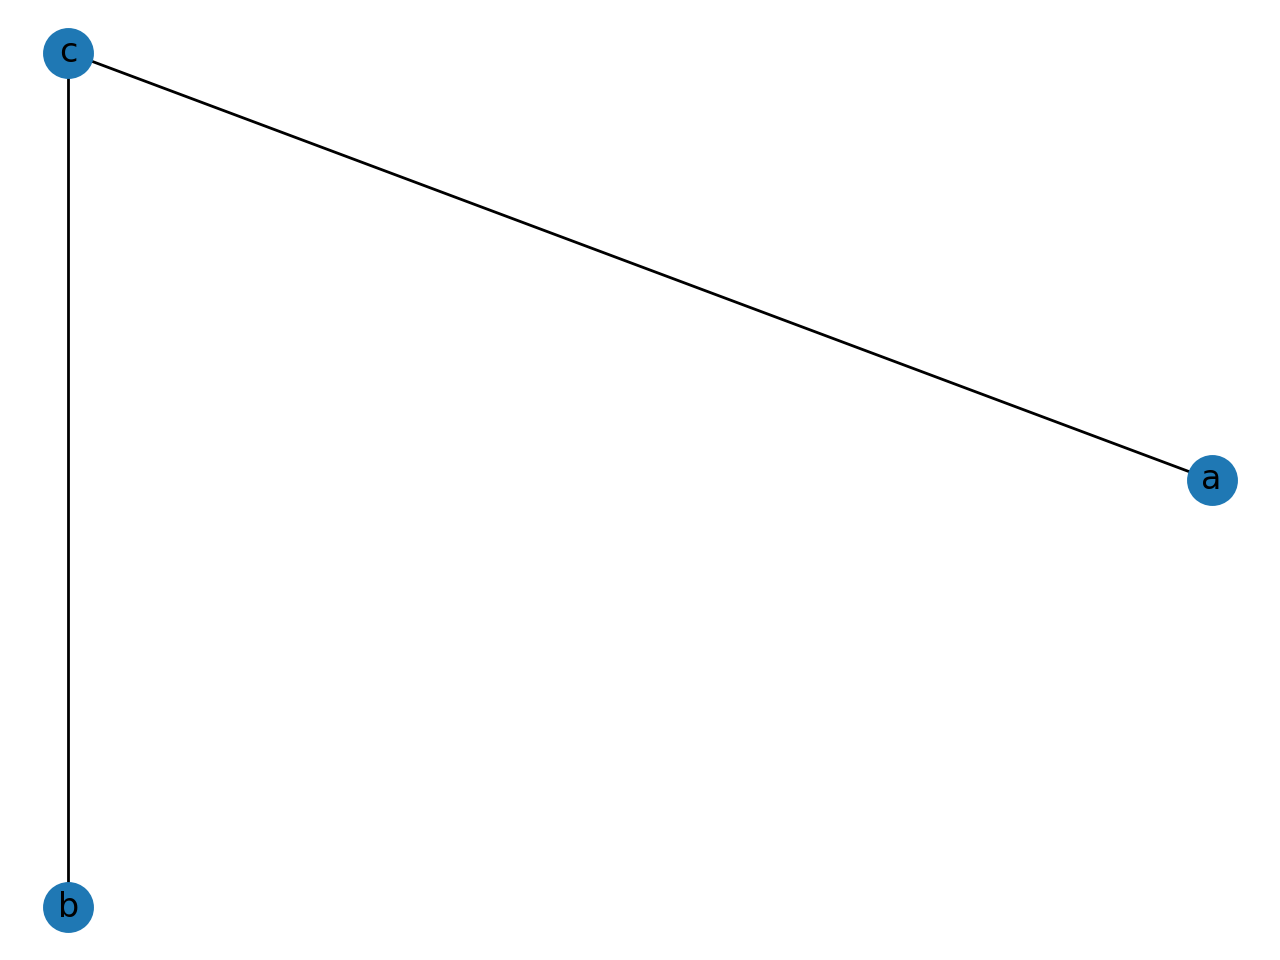
\includegraphics[width=\linewidth]{DTM1.png}}
\caption{An example demonstrating the non-sobmodularity of the DTM model. Nodes $a$ and $b$ have threshold 1, and node $c$ has threshold 2.}
\label{fig:DTM1}
\end{figure}
\subsubsection{Applications}
TBPI can be readily applied to optimize marketing campaigns by companies. In a marketing campaign, one can hand down discount vouchers to users to convert them. These vouchers are the unit of incentive that can be assigned. The outcome of the campaign is then measured a limited amount of time after the campaign has started, as many products become irrelevant in time for any number of possible reasons.
\subsection{Gargano et al. \cite{gargano}}
In \cite{gargano}, Gargano, Hell, Peters, and Vaccaro introduce the concept of limited active-time for nodes previously mentioned in section \ref{sec:LAT-dim}. We will refer to this model as Limited-Active-Time henceforth and abbreviate it as LAT.
\subsubsection{Limited-Active-Time (LAT)}
Once activated, nodes remain influenced forever, but are active only for a fixed number of rounds, $\lambda$. I.e. they only influence their neighbours for $\lambda$ rounds only after their initial activation. LAT is a deterministic model based on DTM with the same threshold-based activation mechanism. \\
An interesting research direction yet unexplored in the literature, could be to extend the limited active-time concept to other models besides the deterministic threshold model -- e.g. to the probabilistic LT model where the modification would be fairly straightforward. \\
LAT is \textbf{non-monotone}, \textbf{non-submodular} and also \textbf{non-timing-insensitive}. Figure \ref{fig:LAT1} is a counter-example demonstrating that LAT does not have any of the properties outlined for diffusion models. -- Adding node $b$ to the seed set $\{a\}$ will result in a decrease in the spread function. Adding $d$ to the resulting set, $\{a, b\}$, will yield an increase; thus, demonstrating non-monotonicity of the model. Non-submodularity can be shown by adding $b$ to the seed $\{a, c\}$ and observing the increase in the spread; putting this in contrast with the decrease resulting from adding $b$ to the seed $\{a\}$, rules out submodularity. Also, adding $b$ to $\{a\}$, but in the second round, will not result in a decrease of the final spread, thus, also ruling out timing-insensitivity.
\begin{figure}
\fbox{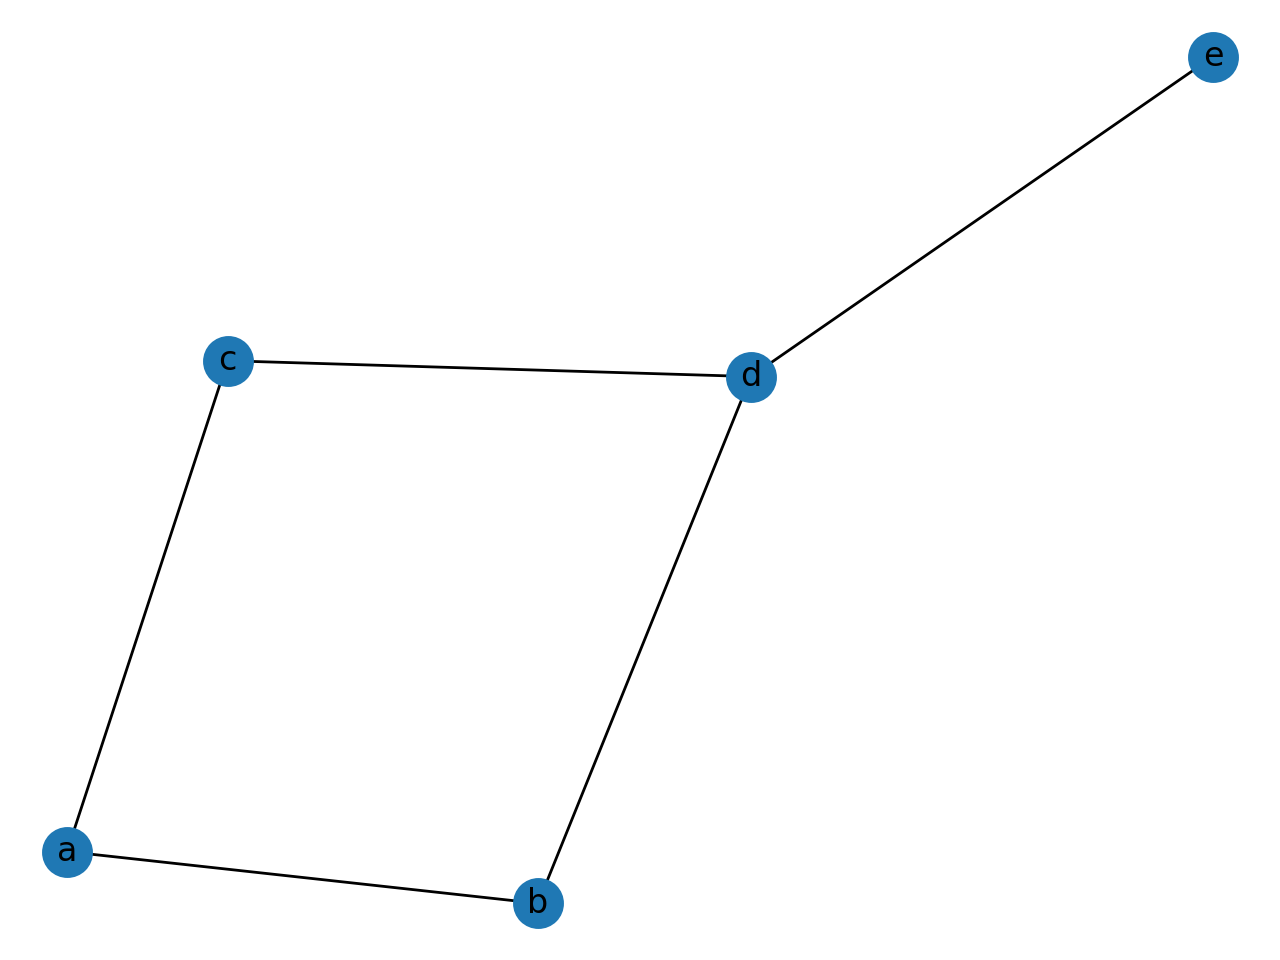
\includegraphics[width=\linewidth]{LAT1.png}}
\caption{Example demonstrating the non-monotonicity, non-submodularity and non-timing-insensitivity of LAT. All nodes have a limited active-time of 1. Nodes $a$ and $d$ have threshold 2, and nodes $c$, $b$ and $e$ have threshold 1.}
\label{fig:LAT1}
\end{figure}
\subsubsection{Applications}
The LAT model is applicable whenever nodes in the network only actively influence their neighbours for a limited time, but still remain under the influence, e.g. the "hype" in a customer for a certain product/brand dies out after a certain amount of time and they don't actively endorse the product even though they might\footnote{This is yet another potential research direction -- a model where the active time is limited for all nodes and influence is persistent for some, and temporary for others. The objective would be to maximize the number of nodes with persistent influence -- i.e. permanent adopters of the product; This would provide a more accurate modeling of the application mentioned for LAT.} continue to use it.
\subsection{Karimi et al. \cite{karimi}}
Emanating from a different background, in \cite{karimi}, Karimi and Holme introduce a conceptually different model of influence diffusion from the previously cited works -- although, concretely, we still have a similar process. They introduce a temporal model where node activations are based on the fraction of their neighbours that are activated within a time window: Fractional-Time-Window (FTW).
\subsubsection{Fractional-Time-Window (FTW)}
FTW is based on a model for social behavior proposed by Granovetter in \cite{grano}, which asserts that \textit{social collective behavior could be divided into processes depending on credulity (including threshold models) or vulnerability (like disease-spreading models)}\cite{karimi}. FTW is an extension of the threshold model proposed by Watts in \cite{duncan}, that is an analytically tractable formulation -- Karimi and Holme augment this model with temporal aspects: \\
FTW is a deterministic temporal model -- nodes can only influence each other at specific \textit{points of contact} throughout the diffusion process; neighbours of a node are defined as those which have at least one point of contact with the node in question. The complete diffusion dynamics of FTW are based on an alternative view on time windows in Gargano et al.'s LAT \cite{gargano}, i.e. its inverse: instead of limiting the window during which a node can \textit{send} its influence to its neighbours, they limit the time a node can \textit{accumulate influence received} from its neighbours; we will term these, \textbf{accumulation-time-windows} in this article. A node is activated once its received influence, during an accumulation-time-window -- i.e. the number of its neighbours the node has point of contact with within its accumulation-time-window -- divided by its total number of neighbours exceeds its \textit{fractional threshold}. \\
Absolute-Time-Window (ATW) \cite{karimi} is an analogous model with absolute thresholds instead of fractional ones -- a generalization of DTM with accumulation-time-windows and edge-presence-times. It is easy to see that this FTW and ATW are equivalent: multiplying the fractional threshold of each node in FTW by the total number of its neighbours gives its absolute threshold in ATW; the inverse transformation is equally trivial. \\
By a simple inductive argument, it is easy to see that these models are \textbf{monotone}: if in one length-$i$ activation sequence $L$, a node is activated by round $i$, it is activated by round $i$, in any other activation sequence $L'$ of the same length, where the set of active nodes in $L'$ is a superset of those in $L$, in all rounds. Taking the active nodes at round $0$, i.e. the seed set as base of induction gives us the desired result. \\ 
DTM can be reduced to ATW, and consequently FTW, by taking the contact points for all edges to consist of all rounds and taking the time window to be infinite, thus ATW, and consequently FTW, are also \textbf{non-submodular} and \textbf{non-timing-insensitive}.
\subsubsection{Applications}
The model in \cite{duncan}, which FTW introduces temporal aspects into, is most suitable to model social influence in social collective behaviour, e.g. adoption of political standpoints through social influence, etc. Although, the fractional nature of the thresholds in FTW make its application to any real-world scenario questionable: the fractional threshold is based on the total number of nodes a node has points of contact with throughout the whole process. This in turn requires nodes to "see into the future" to determine their concrete threshold.
\section{Karp et al. \cite{karp}}
Karp, Schindelhauer, Shenker, and V\"ocking introduce a model for broadcasting which is just as well applicable to influence diffusion with some modification: Random-Phone-Call (RPC)
\subsubsection{Random-Phone-Call (RPC)}
RPC is a discrete time and edge-centric-activation model -- at each step, each node picks up the phone and calls a random neighbour; if any of the nodes at the ends of the phone call is active, they both become activated by the end of that round. \\
In the original model of \cite{karp}, nodes choose randomly between all the nodes in the graph; this reduces to taking to the input graph to be complete in the preceding formulation. As this work comes from a different background, the problem and the optimization objectives are somewhat different -- they show that it takes $O(\ln n)$ rounds asymptotically, for a piece of information originating at one node to reach all other nodes. Although, it should be mentioned again that they assume the underlying graph to be complete, thus enabling all nodes to potentially communicate with each other. Where as in contrast, in influence diffusion problems, the input graph is the main variable of the problem.
\subsubsection{Influence-Diffusion-RPC (IDRPC)}
IDRPC is a model we propose as an extension to RPC, framing it in an influence diffusion context. \\
Karp et al. limit their study to a single initiating node, and focus on the time it takes for a rumour started at one node to spread across the whole network. Note that this always happen with probability 1 as a large number of rounds is passed, as the underlying graph is presumed to be complete -- i.e. any player can call any player. To frame this in an influence diffusion context, and specifically influence maximization, we propose two modifications to the original model: 1. the underlying graph is no more presumed to be complete -- i.e. nodes can only call their neighbours in the given input graph 2. a time limit is enforced on the diffusion process. Modifying the model in this way we obtain an influence maximization problem, and more specifically, a spread function as a function of the seed nodes. \\
It is easy to see that IDRPC is \textbf{monotone}. It is also \textbf{submodular} and \textbf{timing-insensitive}. The timing insensitivity of activations is readily apparent through a simple obeservation: fixing an outcome of the random process, i.e. who calls who, and taking $A_i$, $A'_i$, where $A_i \subseteq A'_i \subseteq V$, the set of active nodes at round $i$ in two different runs of the same process -- i.e. same random outcomes but different seed sequences--, then $A_j \subseteq A'_j$ for all rounds $j \geq i$. In this way, if we move activation of any node $v$ from round $i'$ forward to an earlier round $i$, the set of active nodes in this new process at round $i$, will be a superset of the original process -- where $v$ would have been activated at round $i'$ --, satisfying the predicate for the previous observation, and thus, only increasing the number of active nodes at each round subsequently. \\
To prove the submodularity, we use an argument similar to that of \cite{kempe} for proving the submodularity of the IC model. Again, we fix the random outcomes. For any seed set $S$, a node $u$ will be active by the end of the process, i.e. before the time limit, if there is a temporal journey from any of the nodes in the seed set $u$, to $v$. Framing the problem in this way, it is easy to see that the sufficient and necessary condition for submodularity is satisfied for any random outcome -- the difference adding a node $v$ to a seed set $S$ makes in the spread function, is exactly equal to the size of the set consisting of nodes that have a temporal path from $v$, $P_v$, but not from any of the nodes $u \in S$, $P_S$, i.e. $\sigma(S \cup \{v\}) - \sigma(S) = |P_v / P_S|$. If $S \subseteq S'$, then $P_S \subseteq P_{S'}$, and thus $P_v / P_{S'} \subseteq P_v / P_S$; satisfying submodularity $\sigma(S \cup \{v\}) - \sigma(S) \geq \sigma(S' \cup \{v\}) - \sigma(S')$ for all $S \subseteq S' \subseteq V$ and $v \in V$.
\subsubsection{Applications}
Motivation for this model comes from network sciences. Primarily, it is a robust mechanism for broadcasting in networks.
\subsection{Gayraud et al. \cite{gay}}
Gayraud et al. introduce dynamicity into the underlying graph. They use introduce a pair of distinct mechanisms, \textit{Transient} and \textit{Persistent}, to adapt the diffusion models IC and LT to dynamic, or using \cite{gay}'s terminology, \textit{evolving}, graphs; resulting in the Transient/Persistent-Independent-Cascade (T/PEIC), and Transient/Persistent-Linear-Threshold (T/PELT) models.
\subsubsection{Evolving-Independent-Cascade(T/PEIC))}
In the IC model, nodes get one chance at activating their inactive neighbours: once they are activated, they attempt to activate each inactive neighbour according to the probability assigned to the edge connecting the two nodes. \\ 
In the dynamic case, nodes have different sets of neighbours at different time; there are two straight-forward approaches we can take, to make IC applicable in the context of evolving graphs. \\
\textbf{Transient-Evolving-Independent-Cascade(TEIC)} \\
In the transient setting, if activated at round $i$, nodes will attempt to activate their inactive neighbours of/in round $i+1$, and no more activation attempts is made on their part. \\
\textbf{Persistent-Evolving-Independent-Cascade(PEIC))} \\
In the persistent setting, nodes will not only attempt to activate their inactive neighbours of round $i+1$, but they also make activation attempts at nodes they come in contact with after round $i+1$ at their first point of contact.
\subsubsection{Evolving-Linear-Threshold(T/PELT))}
In the LT model, nodes have a random threshold and they are activated once the total weight of the edges incoming from their active neighbours exceeds that threshold. \cite{gay} frames the Persistent and Transient mechanisms for the LT model as follows.\\
\begin{minipage}{\textwidth}\textbf{Transient-Evolving-Linear-Threshold(PELT)}\end{minipage}\\
This setting corresponds to viewing each snapshot of the evolving graph independently and applying LT on it, i.e. a node is activated at round $i+1$, if the total weight of the incoming edges at round $i$ is greater than its threshold.\\
\begin{minipage}{\textwidth}\textbf{Persistent-Evolving-Linear-Threshold(PELT)} \end{minipage}\\
In the persistent setting, incoming weights from active neighbours are accumulated over time, i.e. a node is activated at round $i+1$, if the total weight of the active edges it has been in contact up to and including round $i$ exceeds its threshold.
\subsubsection{Applications}
Dynamic models are especially applicable to graphs representing networks of social nature. They can be said to be more realistic models than their static counterparts as real-world graphs; especially those in the context of online social networks due to their highly dynamic nature.
\subsection{Bharathi et al. \cite{bhar}}
The models we have introduced so far have all been single-agent models, i.e. a single influence-\textit{type} diffusing over the network. The goal is usually how to choose the initial set of active nodes so as to maximize the number of influenced nodes by the end of the process. \\
Bharathi, Kempe and Salek are the first to introduce additional influencing \textit{agents} into the process, each spreading their own influence-type over the network. They extend and modify the IC model to the multi-agent case: Competitive-Independent-Cascade (CIC).
\subsubsection{Competitive-Independent-Cascade (CIC)}
Competitive-Independent-Cascade (CIC) is a model in which multiple agents (players) start  a diffusion process according to a \textit{continuous} analog of the IC model. The continuous aspect of the model is introduced as a tie-breaking, or rather, tie-prevention, policy for multiple agents trying to activate the same node.
When node $u$ becomes active at time $t$, it attempts to activate each currently inactive neighbor $v$. If the activation attempt from $u$ on $v$ succeeds, $v$ will become active, and of the same \textit{color} as $u$, at time $t+T_{uv}$ if it hasn't been colored by that time, where $T_{uv}$ are independent and exponentially distributed continuous random variables. -- As the probability of activations from different sources occuring at exactly the same time is 0 in this scheme, it prevents competing nodes from attempting to activate an incative node at the same time, thus preventing conflicts.\\
They frame the influence maximization problem in this setting as a game, and offer best strategies for players in two different game settings: 1. In a diffusion with $n$ players, maximize the spread for the $n$th player given the strategies of the previous $n-1$ players. 2. First-mover strategy for a game with 2 players, i.e. for the first player choosing their seed set.
\subsection{Viglietta \cite{vig}}
In \cite{vig} introduces yet another model with a novel modification on the diffusion process -- Subscription Model (SM).
\subsubsection{Subscription Model (SM)}
In SM, similar to LAT, nodes remain active for a limited amount of time, unlike LAT however, it's not just the \textit{active}-time, that is limited, but nodes also lose their \textit{influenced} state once the time-limit, or -window in this case, is passed and their activation threshold is no more satisfied. This mechanism for \textit{internal node influence-retention} was previously introduced in the model dimensions section as the \textit{non-persistent} influence-retention mode. \\
SM is a deterministic model and an extension of DTM: in addition to the dynamics in DTM, nodes are associated with an activation-time-window $\lambda$, where they remain active for $\lambda$ rounds after their activation-threshold is satisfied; after the $\lambda$ rounds have passed however, they will be deactivated as soon as their activation-threshold is not satisfied anymore.
Node activations in this model display interesting and curious properties; they either reach a steady state or are periodic -- they must be periodic if they don't reach a steady state, as the collective-activation-state of the network, the combination of the activation-state of all the nodes in the network that is, takes a limited number of values; and this is keeping in mind that nodes having been activated before can be reactivated if their Viglietta studies throws a deeper glance on these activation-periods for different values of $\lambda$: for $\lambda = 1$, only a period of 2 is possible; if $\lambda > 1$, any period greater than $\lambda$ is possible \cite{vig}. \\
With regards to the properties of influence diffusion models, it is not straightforward to classify this model accordingly: the fact that the influenced-state of nodes might not reach a steady-state, makes the spread-function according to its original definition unapplicable. Thus properties of the spread-function, i.e. properties of the model, become irrelevant. Thus, we will modify the definition of the spread function accordingly as \textit{the number of nodes \textbf{permanently} active, by the time the process has reached a steady-state, or has obtained periodic activations}.\\
This defenition of the spread function falls closely in-line with the concept of self-supporting sets introduced in \cite{vig}: \textit{We call a set of nodes $W \subseteq V$ self-supporting if each node of $v \in W$ has a number of neighbors in W that is at least as large as its threshold $t(v)$\cite{vig}}. Note that self-supporting sets are not necessarily disjoint. Thus, the spread-function in the context of SM can be reformulated as, $\sigma(S)$, \textit{the maximum number of nodes in the union of the self-supporting sets active in a diffusion process starting from the seed set $S$}. Note that we do not mention the time the network has reached steady-state/periodicity in this definition as in the previous formulation; that is implicit in taking the maximum in the self-supporting sets, since self-supporting sets do not undergo state-changes once they are activated. Thus, we have a spread-function for SM, which we can evaluate in terms of the monotonicity, submodularity, and time-insensitivity properties.


it turns out that node-activations are monotonic after $\lambda$ rounds are past in a diffusion process where the underlying graph is complete and hence the steady-state is certain to be attained. Thus, on complete graphs we can maintain our original definition of the spread-function: the number of (permanently) active nodes at the end of the process. 



\begin{thebibliography}{1}

\bibitem{dom} Domingos, Pedro, and Matt Richardson. "Mining the network value of customers." Proceedings of the seventh ACM SIGKDD international conference on Knowledge discovery and data mining. ACM, 2001.
\bibitem{kempe} Kempe, David, Jon Kleinberg, and Éva Tardos. "Maximizing the spread of influence through a social network." Proceedings of the ninth ACM SIGKDD international conference on Knowledge discovery and data mining. ACM, 2003.
\bibitem{kempe0} Kempe, David, Jon Kleinberg, and Éva Tardos. "Maximizing the Spread of Influence through a Social Network." Theory of Computing 11.1 (2015): 105-147.
\bibitem{gargano} Gargano, Luisa, et al. "Influence diffusion in social networks under time window constraints." Theoretical Computer Science 584 (2015): 53-66
\bibitem{cordasco} Cordasco, Gennaro, et al. "Time-Bounded Influence Diffusion with Incentives." International Colloquium on Structural Information and Communication Complexity. Springer, Cham, 2018.
\bibitem{karimi} Karimi, Fariba, and Petter Holme. "Threshold model of cascades in temporal networks." arXiv preprint arXiv:1207.1206 (2012).
\bibitem{grano} Granovetter, Mark. "Threshold models of collective behavior." American journal of sociology 83.6 (1978): 1420-1443.
\bibitem{duncan} Watts, Duncan J. "A simple model of global cascades on random networks." Proceedings of the National Academy of Sciences 99.9 (2002): 5766-5771.
\bibitem{karp} Karp, Richard, et al. "Randomized rumor spreading." Proceedings 41st Annual Symposium on Foundations of Computer Science. IEEE, 2000.
\bibitem{gay} Gayraud, Nathalie TH, Evaggelia Pitoura, and Panayiotis Tsaparas. "Diffusion maximization in evolving social networks." Proceedings of the 2015 acm on conference on online social networks. ACM, 2015.
\bibitem{bhar} Bharathi, Shishir, David Kempe, and Mahyar Salek. "Competitive influence maximization in social networks." International workshop on web and internet economics. Springer, Berlin, Heidelberg, 2007.

\end{thebibliography}


\end{document}



